\documentclass{article}
\usepackage{listings}
\usepackage{graphicx}
\usepackage[slovene]{babel}
\usepackage{color}
\usepackage{amsmath}
\usepackage[usenames,dvipsnames]{xcolor}
\usepackage[hidelinks]{hyperref}
\usepackage{subcaption}
\usepackage{float}
\usepackage{rotating} 
\usepackage{hyperref}
\usepackage{caption}
\graphicspath{{./images/}}

\setlength{\parindent}{0pt}

\newcommand{\MAD}{\mathrm{MAD}}


\begin{document}

\title{Matematično-fizikalni praktikum \\[3mm] \large Naloga 1}
\author{Luka Papež}
\date{16.\ oktober 2024}

\begin{center}
    
\includegraphics[width=8cm]{logo-fmf.png}
\end{center}

{
    \let\newpage\relax
    \maketitle
}

\maketitle
\newpage
\section{Naloga}
{\sl Naloga:} Napravi računalniško simulacijo
dvorazsežne naključne hoje za \textbf{polete in sprehode}.  Začni vedno v izhodišču
($x=y=0$), nato pa določi naslednjo lego tako, da naključno
izbereš smer koraka in statistično neodvisno od te izbire
še njegovo dolžino, torej
\begin{eqnarray*}
x &\leftarrow& x + l \cos\phi \>, \\
y &\leftarrow& y + l \sin\phi \>,
\end{eqnarray*}
kjer je $\phi$ enakomerno naključno porazdeljen po intervalu
$[0,2\pi]$, dolžina koraka $l$ pa naj bo porazdeljena
v skladu s potenčno obliko. 
Dolžine $l_i$ je v tem primeru potrebno generirati po verjetnostni
porazdelitvi w(l)$\sim$ p(l).

V vsakem primeru nariši nekaj značilnih slik sprehodov za $10$, $100$, $1000$ in $10000$ korakov. Iz velikega števila sprehodov z velikim številom korakov nato poskusi določiti eksponent $\gamma$ za nekaj izbranih parametrov $\mu$ oziroma funkcij $f(x)$ v posameznih primerih ter presodi, za kakšno vrsto difuzije gre.


\section{Uvod}
Naključni sprehodi so vrsta gibanja, pri katerem
v velikem številu korakov napredujemo iz izhodišča
v neko končno lego, tako da se parametri vsakega naslednjega
koraka sproti naključno določajo.  Običajni zgled
je Brownovo gibanje (difuzija) drobnih delcev barvila
po mirujoči homogeni tekočini, kjer je spočetka barvilo
zbrano v izhodišču.  ``Težišče'' barvila
$\langle x(t)\rangle$ v povprečju ostane v izhodišču,
razen če v tekočini vzpostavimo kako anizotropijo (na primer
v dveh razsežnostih z vsiljeno rotacijo).  ``Razmazanost''
po dolgem času je sorazmerna s časom,
\begin{equation*}
  \sigma^2(t) \equiv \langle x^2(t)\rangle - \langle x(t)\rangle^2 = 2 D t \>.
\end{equation*}
Sorazmernostni koeficient je običajna difuzijska konstanta,
priča smo normalni difuziji.  Ta rezultat izhaja iz
centralnega limitnega teorema (CLT), ki izraža,
da je rezultantna porazdelitev končnih leg pri difuziji
porazdeljena normalno (Gauss), če so le povprečni časi
med koraki in povprečni kvadrati dolžin korakov končni.

Zanimiveje je opazovati naključne sprehode, pri katerih dovolimo
nadpovprečno dolge korake.  Verjetnostno gostoto porazdelitve
po dolžinah posameznih korakov parametrizirajmo v potenčni obliki
\begin{equation}
p(l) \propto l^{-\mu} \>,
\label{lpow}
\end{equation}
kjer naj bo $1 < \mu < 3$.  Tedaj postane drugi moment porazdelitve
\begin{equation*}
  \langle l^2\rangle = \int l^2 p(l) l
\end{equation*}
neskončen.  Govorimo o anomalni difuziji, prisotni pri celi dru\v zini
kinematičnih distribucij dolžin poti z "debelimi repi".

Ustrezno sliko naključnega gibanja, povezanega s temi dolgimi koraki, lahko
interpretiramo na dva načina:
\begin{itemize}
  \item L\'evyjev pobeg oz. polet ({\sl flight\/}), implicira, da vsak korak iz
  porazdelitvetraja enako dolgo, medtem ko se hitrost gibanja med koraki (divje) spreminja.
  \item L\'evyjev sprehod ({\sl walk\/}), ki interpretira korak iz porazdelitve kot  gibanje s konstantno hitrostjo in
  tako koraki trajajo različno dolgo časa (dolžina koraka je sorazmerna s časom).
\end{itemize}

Slednja intepretacija bolj ustreza fizikalni sliki naključnega gibanja delca skozi snov, medtem ko
se prva interpretacija uporablja v druga\v cnih aplikacijah.

Vse naloge lahko obravnavaš za obe interpretaciji, pobegov in sprehodov. V prvem primeru (pobeg, flight) je
prete\v ceni \v cas direktno sorazmeren s \v stevilom korakov, v drugem primeru (sprehod, walk) pa je
prete\v ceni \v cas  sorazmeren z vsoto dol\v zine korakov.


Pri anomalni difuziji razmazanost (varianca) velike množice
končnih leg naključnih L\'evyjevih \textbf{sprehodov (walks)} narašča z drugačno potenco časa.
Velja $\sigma^2(t) \sim t^\gamma$, kjer je
\begin{align*}
1 < \mu < 2 \>, &\qquad \gamma = 2 \> &\qquad&  \text{(balistični režim)}\>, \\
2 < \mu < 3 \>, &\qquad \gamma = 4 - \mu &\qquad&  \text{(super-difuzivni režim)}\>, \\
    \mu > 3 \>, &\qquad \gamma = 1 &\qquad&  \text{(normalna difuzija)} \>.
\end{align*}
Za $\mu=2$ pričakujemo $\sigma^2(t) \sim t^2 / \ln t$,
za $\mu=3$ pa $\sigma^2(t) \sim t \ln t$ (glej na primer \cite{weeks}
in druge reference prav tam).

Slika je nekoliko drugačna pri opazovanju naključnih L\'evyjevih \textbf{poletov (flights)}.
Spet vzamemo zvezo $\sigma^2(t) \sim t^\gamma$ in dobimo odvisnosti
\begin{align*}
1 < \mu < 3 \>, &\qquad \gamma = \frac{2}{\mu-1} \> &\qquad&  \text{(super-difuzivni režim)}\>, \\
    \mu > 3 \>, &\qquad \gamma = 1 &\qquad&  \text{(normalna difuzija)} \>.
\end{align*}
Pri $\mu=2$ očitno pričakujemo $\sigma^2(t) \sim t^2 $, torej balistični režim.
\newline


{\sl Statistični komentar:} v primerih, ko je drugi
moment porazdelitve neskončen, bo tudi račun razmazanosti
končnih leg $x_n$ v obliki
\begin{equation}
\sigma^2 = \frac{1}{N-1} \sum_{n=1}^N \left( x_n - \langle x \rangle \right)^2
\label{sig2}
\end{equation}
divergiral oziroma bo imel ob ponovnih zagonih naključnega sprehoda
močno raztresene vrednosti. Ta problem rešimo z uporabo robustne mere MAD,
``median absolute deviation''
\begin{equation*}
  \mathrm{MAD} \equiv \mathrm{median}_i\left( | X_i - \mathrm{median}_j X_j | \right) \>.
\end{equation*}
Z njo merimo povprečje absolutne vrednosti deviacije na način,
ki je zelo malo občutljiv na oddaljene vrednosti v repih porazdelitve,
saj te vrednosti na račun mediane bistveno manj vplivajo kot na
račun običajne povprečne vrednosti.

\section{Rešitev}
\subsection{Naključna pot}
Za generiranje naključnih poti moramo najprej določiti porazdelitev po kateri bomo računali dolžino koraka. V navodilih imamo podano sorazmerje $w(l) \propto p(l) \propto l^{-\mu}$, ter enačbo,
\begin{equation*}
  \int\limits_{a}^{l} w(t)\,  dt = \rho \cdot \int\limits_{a}^{b}  w(t)\, dt,
\end{equation*}
kjer je $\rho \in [0, 1]$, $a$ in $b$ pa spodnja in zgornja meja. Iz te elegantne zveze dobimo predpis za generiranje naključne razdalje pri izbrani porazdelitvi. 
\begin{equation*}
    l = (\rho b^{1 - \mu} + (1 - \rho) a^{1 - \mu})^{\frac{1}{1 - \mu}}
\end{equation*}
Da se izognemo težavam s konvergenco integralov nastavimo $a=1$ in izlimitiramo b v neskončnost. To nam da izraz
\begin{equation*}
  l = (1 - \rho)^{\frac{1}{1 - \mu}}
\end{equation*}
Za generiranje kota premika pa preprosto uporabimo uniformno porazdelitev. Da preverimo formulo narišimo histogram porazdelitev
\begin{figure}[H]
  \centering
  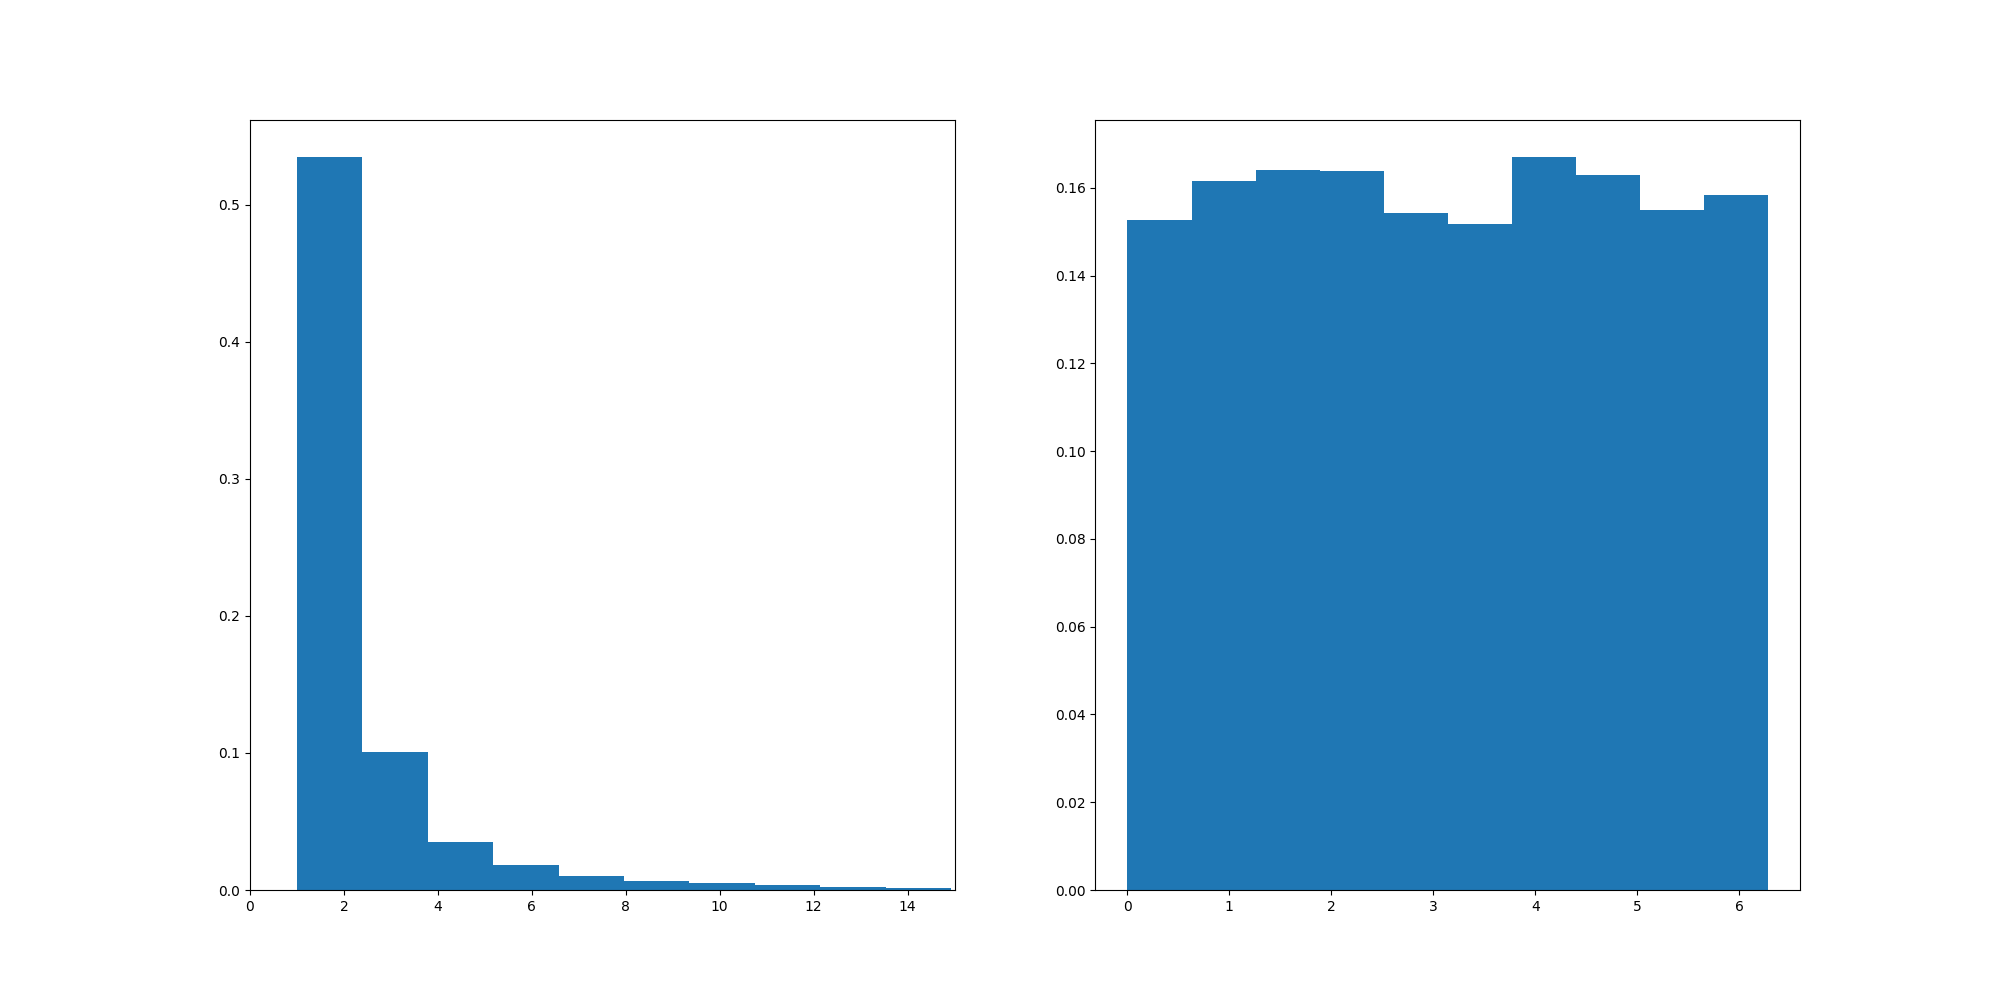
\includegraphics[width=1\textwidth]{distribution.png} 
  \caption{Distribucija dolžine (levo) in kotov (desno) koraka pri $\mu = 2.5$}
\end{figure}
Kot vidimo obe porazdelitvi ustrezata pričakovani obliki. Zato lahko za začetek narišemo nekaj poti pri $\mu = 2.5$
\begin{figure}[H]
  \centering
  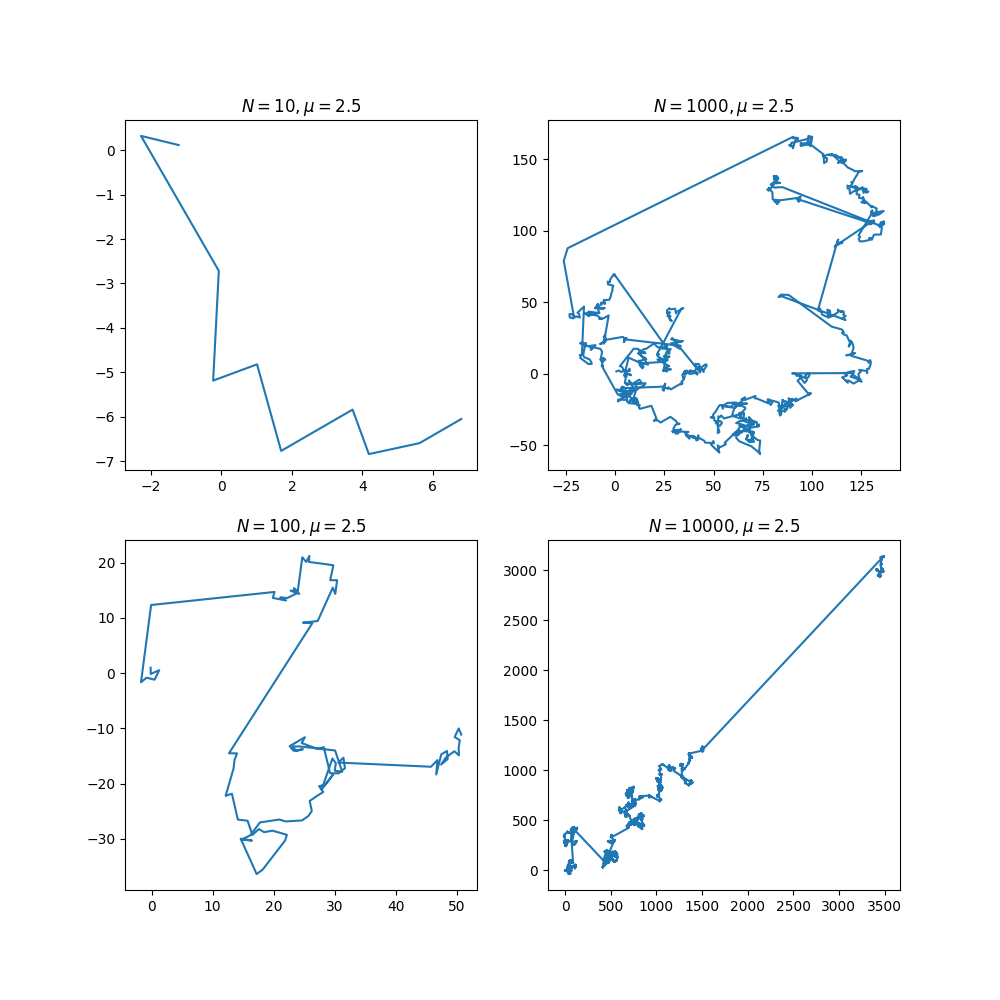
\includegraphics[width=1\textwidth]{nice_plots.png} 
  \caption{Naključne poti pri $\mu = 2.5$}
\end{figure}

\subsection{L\'evyjev polet in sprehod}
Zdaj imamo vse potrebne pogoje za obdelavo razmazanosti. Kot že omenjeno v uvodu bomo to računali s pomočje mere MAD, ki je sorazmerna s standardno deviacijo in sicer $\MAD \approx 0.6745 \sigma$ \cite{wiki}. Standardna deviacija pa je koren variacije. Tako smo robustno izračunali variacijo, ki je sorazmerna s potenco časa $\sigma^2 \propto t^\gamma$. Iz tega razmerja lahko potem iz dveh točk določimo $\gamma$
\begin{equation*}
  \gamma = \frac{\log(\sigma_2) - \log(\sigma_1)}{\log(t_2) - \log(t_1)}
\end{equation*}
Ta postopek nato iteriramo čez več točk in s tem določimo povprečno $\gamma$ in napako fita. L\'evyjevi poleti so čeprav fizikalno manj smiselni preprostejši za implementacijo, saj je čas direktno sorazmeren s številom korakov. Zato bomo začeli z njimi in narisali  odvisnost $\sigma^2$ od časa. 

\begin{figure}[H]
  \centering
  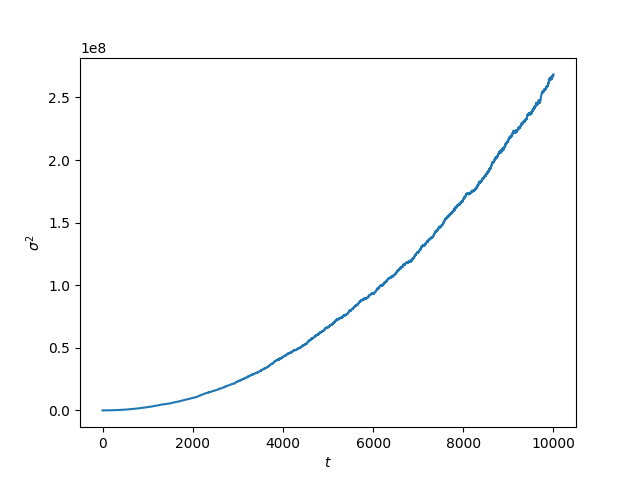
\includegraphics[width=0.8\textwidth]{vartimemu2.png} 
  \caption{Odvisnost variacije od časa pri $\mu=2$}
\end{figure}
Pričakovano glede na podano teorijo opazimo potenčno funkcijo. 
Zdaj pa si poglejmo, kar odvisnost $\gamma$ od $\mu$ za L\'evyjeve polete. Pri risanju grafa izvedemo tisoč poletov z deset tisoč koraki in to ponovimo desetkrat. 
\begin{figure}[H]
  \centering
  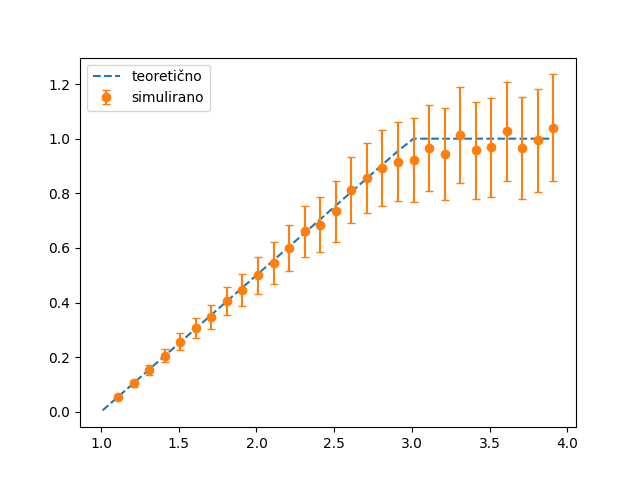
\includegraphics[width=0.9\textwidth]{gammamuflights.png} 
  \caption{Odvisnost $\gamma$ od $\mu$ pri L\'evyjevih poletih}
\end{figure}
Naša simulacija je bila precej uspešna. V intervalu super-difuzije so razlike minimalne. Odstopanja opazimo predvsem okoli $\mu=3$ torej na prehodu med super-difuzivnim načinom in normalnim. To je najverjetneje posledica nezveznosti teoretične funkcije v tej točki. Z več iteracijami in koraki pa bi se najverjetneje ta odstopanja zmanjšala.\\
V drugem delu naloge pa sledijo še L\'evyjevi sprehodi. Za te smo uporabili implementacijo poletov in nato razbili točke tako, da je čas sorazmeren s prepotovano razdaljo. Ker za izračun $\MAD$ potrebujemo pozicije ob enakem času je to precej bolj časovno zahtevno. Zato bomo vzeli le tisoč sprehodov s po tisoč koraki in to enako kot prej ponovili desetkrat.
\begin{figure}[H]
  \centering
  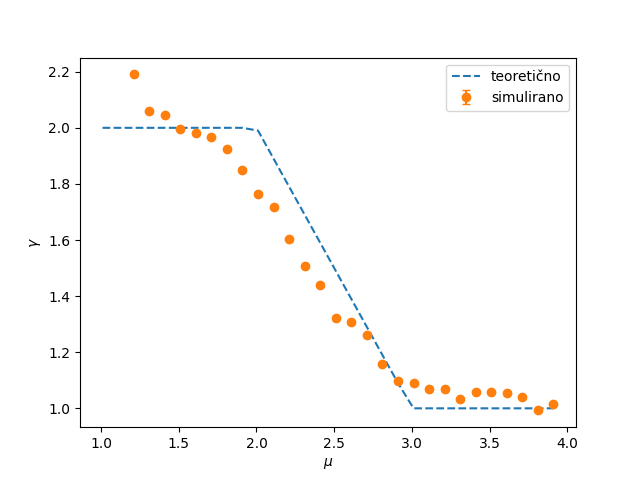
\includegraphics[width=0.9\textwidth]{gammamuwalks.png} 
  \caption{Odvisnost $\gamma$ od $\mu$ pri L\'evyjevih sprehodi}
\end{figure}
Pri sprehodih so razlike večje, a so dobljene napake simulacije presenetljivo majhne. Razlike od teorije lahko pripišemo dejstvu, da smo uporabili manjše število korakov in iteracij. Kljub temu pa je splošen trend teoretične gamme še vedno viden. Odstopanje opazimo pri $\mu=2$, kjer je prehod med balističnim in super-difuzivnim režimom. Pri prehodu v normalni režim pa so nenatančnosti največje kar se verjetno zgodi zaradi premalega števila korakov. 
\newpage
\section{Zaključek}
Sama ideja naloge je precej preprosta. Najtežji del naloge je bila gotovo implementacija L\'evyjevih sprehodov. Lahko bi si sicer ta del naloge še precej utežil z učinkovitim implementiranjem le teh, a se tega zaradi pomanjkanja časa nisem lotil. Največ časa pa sem porabil na iskanju dejstva, da sem uporabljal premajhen interval pri generiranju naključnih razdalj. Za konec pa še zanimivo dejstvo, da je imel \href{https://www.righto.com/2024/08/space-shuttle-interim-teleprinter.html}{Space Shuttle na krovu teleprinter}. 
\begin{thebibliography}{99}
  \setlength{\itemsep}{.2\itemsep}\setlength{\parsep}{.5\parsep}
  \bibitem{weeks} E.~R.~Weeks, J.~S.~Urbach, H.~L.~Swinney, Physica D {\bf 97} (1996) 291.
  \bibitem{wiki} Baccyak4H, Rgbcmy, Median absolute deviation, Wikipedia (2024)
\end{thebibliography}

\end{document}
